%%% LaTeX Template: Article/Thesis/etc. with colored headings and special fonts
%%%
%%% Source: http://www.howtotex.com/
%%% Feel free to distribute this template, but please keep to referal to http://www.howtotex.com/ here.
%%% February 2011
%%%
%%% Modified January 2016 by CDM

%%%  Preamble
\documentclass[11pt,letterpaper]{article}
\usepackage[margin=1.0in]{geometry}
\usepackage[T1]{fontenc}
\usepackage[bitstream-charter]{mathdesign}
\usepackage[latin1]{inputenc}					
\usepackage{amsmath}						
\usepackage{xcolor}
\usepackage{cite}
\usepackage{hyphenat}
\usepackage{graphicx}
\usepackage{float}
\usepackage{subfigure}
\usepackage{sectsty}
\usepackage[compact]{titlesec} 
\usepackage[tablegrid]{vhistory}
\usepackage{pbox}
\allsectionsfont{\color{accentcolor}\scshape\selectfont}

%%% Definitions
\definecolor{accentcolor}{rgb}{0.0,0.0,0.5} 
\newcommand{\teamname}{STEAM}
\newcommand{\productname}{GROCO}
\newcommand{\coursename}{CSE 4316: Senior Design I}
\newcommand{\semester}{Fall 2021}
\newcommand{\docname}{Architectural Design Specification}
\newcommand{\department}{Department of Computer Science \& Engineering}
\newcommand{\university}{The University of Texas at Arlington}
\newcommand{\authors}{Patrick Faulkner \\ Hozefa Tankiwala \\ Andrew Hands \\ Kiran Karki \\ Uyen Do}

%%% Headers and footers
\usepackage{fancyhdr}
	\pagestyle{fancy}						% Enabling the custom headers/footers
\usepackage{lastpage}	
	% Header (empty)
	\lhead{}
	\chead{}
	\rhead{}
	% Footer
	\lfoot{\footnotesize \teamname \ - \semester}
	\cfoot{}
	\rfoot{\footnotesize page \thepage\ of \pageref{LastPage}}	% "Page 1 of 2"
	\renewcommand{\headrulewidth}{0.0pt}
	\renewcommand{\footrulewidth}{0.4pt}

%%% Change the abstract environment
\usepackage[runin]{abstract}			% runin option for a run-in title
%\setlength\absleftindent{30pt}			% left margin
%\setlength\absrightindent{30pt}		% right margin
\abslabeldelim{\quad}	
\setlength{\abstitleskip}{-10pt}
\renewcommand{\abstractname}{}
\renewcommand{\abstracttextfont}{\color{accentcolor} \small \slshape}	% slanted text

%%% Start of the document
\begin{document}

%%% Cover sheet
{\centering \huge \color{accentcolor} \sc \textbf{\department \\ \university} \par}
\vspace{1 in}
{\centering \huge \color{accentcolor} \sc \textbf{\docname \\ \coursename \\ \semester} \par}
\vspace{0.5 in}
\begin{figure}[h!]
	\centering
   	
\includegraphics[width=0.3\textwidth]{images/whiteTeamLogo.png}
\end{figure}
\vspace{0.5 in}
{\centering \huge \color{accentcolor} \sc \textbf{\teamname \\ \productname} \par}
\vspace{0.5 in}
{\centering \large \sc \textbf{\authors} \par}
\newpage


%\vspace{1 in}
%\centerline{January 13th, 2012}
%\newpage

%%% Revision History
\begin{versionhistory}
  	\vhEntry{0.1}{10.29.2021}{PF}{document creation}
  	\vhEntry{0.2}{11.05.2021}{PK|HT|AH|KK|UD}{first draft}
  %	\vhEntry{0.3}{10.12.2015}{AT|GH}{release candidate 1}
  %	\vhEntry{1.0}{10.20.2015}{AT|GH|CB}{official release}
  %	\vhEntry{1.1}{10.31.2015}{AL}{added design review requests}
\end{versionhistory}
\newpage

%%% Table of contents
\setcounter{tocdepth}{2}
\tableofcontents
\newpage

%%% List of figures and tables (optional)
\listoffigures
\listoftables
\newpage

%%% Document sections
\section{Introduction}
%Your introduction should describe your product concept in sufficient detail that the architectural design will be easy to follow. The introduction may include information used in the first sections of your SRS for this purpose. At a minimum, ensure that the product concept, scope and key requirements are described.
Groco is a grocery shopping web application that is accessible on PCs and will be accessible on smartphones, and tablets in the future. Users will be able to search for grocery items and based on the user's brand preference and location, the system will suggest the optimal grocery items. The system also allows users to search for recipes, add their recipes and meal plans into their shopping list to perform the optimization and navigation route.

The purpose of this product is to help users with grocery shopping. The key requirements are:
\begin{itemize}
\item \textbf{The application must allow a user to search grocery items}: A search functionality must be implemented into the application which will allow the user to search for a specific grocery item and then allows the user to add that item to their shopping/grocery list. The user must be allowed to type in the grocery item they are looking for and the search should find the matching item for the user to add to the list.

\item \textbf{The application must present the user with the best grocery item}: Based on the item that the user searched for, the application should go and look for the best possible match for that item based on the price of the item and the location of the stores that item is available in. The application may list multiple options for the same item depending on the item's price and store's location.

\item \textbf{The application must allow users to choose references that define optimal items}: The user should be able to choose the brand, price, distance, and maximum stores preferences for certain grocery items.

\item \textbf{The application must allow users to create grocery lists}: The application must allow users to create shopping lists. The shopping list must store multiple items. The user should be able to add items to their shopping list by searching for the item

\item \textbf{The application must search for all items on the shopping list}: The application must search for all items in the shopping list and return the optimal items, their stores, and their prices based on user-specified preferences

\item \textbf{The application search for optimal items from more than one store}: When the user searches their entire grocery list, the application must search for the optimal results from more than one store.

\item \textbf{The application must provide the most optimal route to the user}: If the user opts to visit multiple stores to get their groceries then the application should provide the user with an optimal route and the order in which the user should visit those stores. The application must consider multiple factors in deciding the route.

\item \textbf{The application must allow users to view and share recipes}: Users should be able to look up recipes in the application. Users must also be allowed to create their recipes and save them. The recipes will store both the ingredients for that recipe and the procedure to follow. Users must be able to view and share recipes with other users.

\item \textbf{The application must allow users to add all ingredients from a recipe to their shopping list}: The application must allow the user to add all the ingredients of a recipe to their shopping list.

\item \textbf{The application must allow users to keep a list of favorite grocery items}: The application must allow users to add and remove grocery items to a favorites list. This will allow users to quickly add certain grocery items to their shopping list.

\end{itemize} 

The key requirement of this product is to optimize the grocery items based on users' preferences. The user's preferences include brand, number of stores, and max traveling distance. The system will choose the optimal item by prices and distance.  

The scope of the product covers grocery stores that have their products and store information online and allow third party access to request or collect data through their public API or web-scraping within the United States. The product prototype should be completed within the budget of 800 dollars and by April 29, 2022.

The main assumptions in this project are that users have internet access, the items' prices and store information collected online are accurate. Groco is not responsible for the price changes or stock-out at the stores. It is the user's responsibility to make sure that a price and discount offer is present at the stores since they are subject to change without notice.

The product contains no obscene material; therefore it is suitable for general grocery shoppers and is made available publicly and free of charge for all users.

The final product will be tested and approved by the client. The development team is free to decide which developing tools and programming languages to be used.


\newpage
\section{System Overview}
%This section should describe the overall structure of your software system. Think of it as the strategy for how you will build the system. An architectural "layer" is the top-level logical view, or an abstraction, of your design. Layers should be composed of related elements of similar capabilities, and should be highly independent of other layers, but should have very clearly defined interfaces and interactions with other layers. Each layer should be identified individually and should be unique as to its function and purpose within the system. This section should also contain the high-level block diagram of the layers, as shown in the example below, as well as detailed descriptions of the functions of each layer.
Groco consists of four main layers: the front-end (the client), the back-end (the server), the database, and the data collector. To create an account and store a user's information, the font end layer will take inputs from the users, send them to the back-end layer to validate, and finally store them in the database. Similarly, the front-end layer will send a request to the back-end and the back-end can retrieve the data from the database then return the appropriate data to display on the front-end. To search for the items, the front-end will take inputs from the users, send them to the back-end layer to process, the back-end will request data from the data collector, using the collected data the back-end complete the request and return the result to display on the front-end. 

\begin{figure}[h!]
	\centering
 	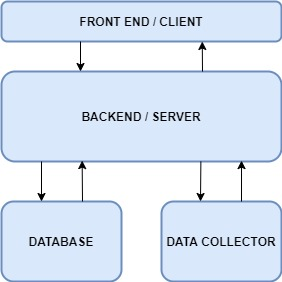
\includegraphics[width=0.4\textwidth]{images/ADS_overview.jpg}
 \caption{A simple architectural layer diagram}
\end{figure}

\subsection{Front-end Description}
%Each layer should be described separately in detail. Descriptions should include the features, functions, critical interfaces, and interactions of the layer. The description should clearly define the services that the layer provides. Also include any conventions that your team will use in describing the structure: naming conventions for layers, subsystems, modules, and data flows; interface specifications; how layers and subsystems are defined; etc. 
The front-end layer includes all software and hardware that is part of a product interface. The hardware includes PC, mobile phones, and tablets. The software is the code that is executed on the client-side (typically HTML, CSS, and JavaScript) that runs in the user's browser to create the user interface. Users interact directly with different components of the front-end, including user-entered data, buttons, links, and other features. The front-end includes subsystems such as login, register, shopping list, recipes, meal planning, and shop. The front-end is designed to be accessible, pleasant, and easy to use.

\subsection{Server Description}
The back-end layer is the code that runs on the server. The back-end receives requests from the front-end (client) and contains the logic of the application to process the request and return the appropriate data to the client. The back-end can directly interact with the database and data collector to retrieve the required data to fulfill the request. The back-end layer includes subsystems such as shopping manager, data parser, user management, query management, and database controller.

\subsection{Database Description}
The database layer stores and retrieves data. The database is also responsible for managing updates. The database layer includes multiple data tables that correspond with different functionalities of the product such as a table for a user, meal plan, shopping list, item, item-brand, brands, recipes, and recipe ingredients.
%Having a separate database layer will allow quick and flexible access to multiple concurrent requests from the webserver. Storing the data in a database also reduces the load on the main memory of the server CPU and provides security, data backup, ensuring the integrity of data, and access to data when the server crashes.

\subsection{Data Collector Description}
The data collector layer is responsible for retrieving data from multiple sources. There is one subsystem in the data collector layer, the API Manager. The data collector retrieves data from various stores through API and returns it to the backend layer.


\newpage
\section{Subsystem Definitions \& Data Flow}
Figure 2 is the data flow diagram for Groco. The diagram shows the Graphical User Interface, Server/Backend, Database, and Data Collector along with their subsystems and the data flow between them. 

\begin{figure}[h!]
	\centering
 	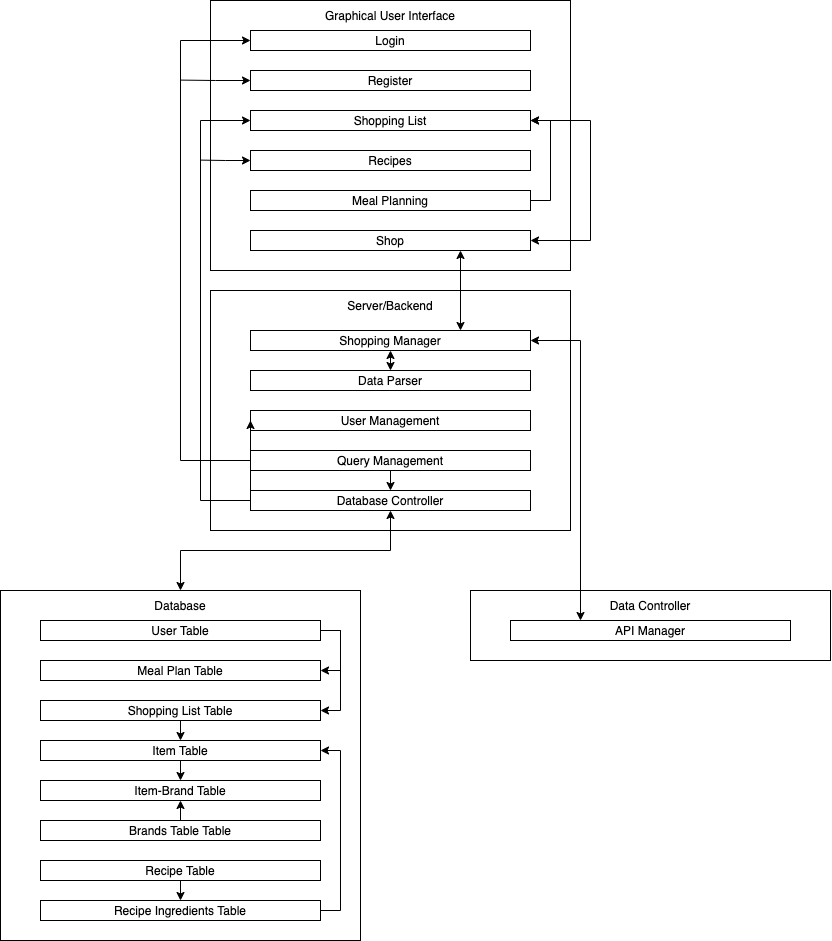
\includegraphics[width=0.5]{images/flowChart}
 \caption{Groco data flow diagram}
\end{figure}
\newpage
\section{X Layer Subsystems}
\subsection{Layer Operating System}
The front-end, like the entire application, will be run on the browser and will therefore run on any operating system.

\subsection{Layer Software Dependencies}
The entire front-end will depend on Bootstrap, and the React library. The front-end will also depend on a consistent connection to the Query Manager on the Server layer.

\subsection{Login Subsystem}
The Login Subsystem will will provide an interface for user to login into the application. Users will be able to login with their email and password credentials or their Google accounts.

\begin{figure}[h!]
	\centering
 	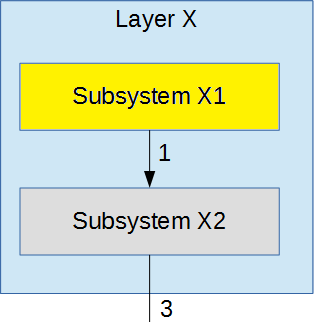
\includegraphics[width=0.60\textwidth]{images/subsystem}
 \caption{Example subsystem description diagram}
\end{figure}

\subsubsection{Subsystem Software Dependencies}
For a user to login with their Google accounts, the Login Subsystem will depend on the GoogleLogin library.

\subsubsection{Subsystem Programming Languages}
The Login Subsystem will be developed using, React.js, HTML, and CSS.

\subsubsection{Subsystem Data Processing}
If the user logs in using their email and password, they will enter their credentials in the respective places and click the login button. Upon the login buttoin being pressed, the Login Subsystem will send the user's credentials to the Query Manager in the backend layer. If the Login Subsystem receives a success signal, then the user will be redirected to the Home Page. If the Login Subsystem receives a failure signal, the Login Subsystem will display a failure message and prompt the user to re-enter their credentials.

If the user decides to login with their Google account, they will select the Google login button. The Login Subsystem will then call on the GoogleLogin API which users will login with. If the login is successful, the Login Subsystem will redirect the user to the Home Page. If the login fails, the user will be given an error message and prompted to re-enter their credentials.

%------------> Register 
\subsection{Register Subsystem}
The Register Subsystem will provide an interface for users to register for an account.

\begin{figure}[h!]
	\centering
 	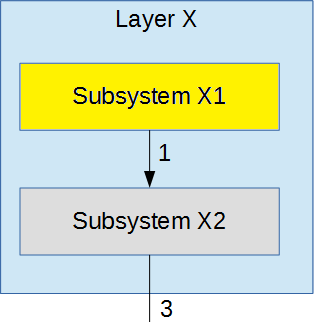
\includegraphics[width=0.60\textwidth]{images/subsystem}
 \caption{Example subsystem description diagram}
\end{figure}

\subsubsection{Subsystem Software Dependencies}
The Register Subsystem does not have any additional dependencies.

\subsubsection{Subsystem Programming Languages}
The Register Subsystem will be developed using, React.js, HTML, and CSS.

\subsubsection{Subsystem Data Processing}
After entering their password and unique email and username, the user will press the Register button. Upon the Register button being pressed, the Register Subsystem will capture the user entered information and send it to the Query Manager. If the Query Manager sends a success signal, the Register Subsystem will redirect the user to the Home Page. If the Query Manager sends a failure signal, the Register Subsystem will display an error message and prompt the user to re-enter their information.

%------------> Shopping List
\subsection{Shopping List Subsystem}

\begin{figure}[h!]
	\centering
 	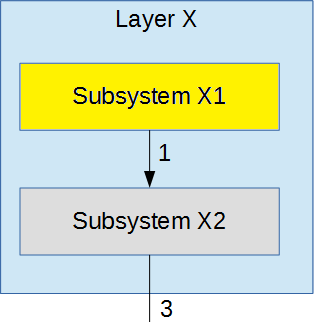
\includegraphics[width=0.60\textwidth]{images/subsystem}
 \caption{Example subsystem description diagram}
\end{figure}

\subsubsection{Subsystem Software Dependencies}
The Shopping List Subsystem has no additional dependencies.

\subsubsection{Subsystem Programming Languages}
The Shopping List Subsystem will be developed using, React.js, HTML, and CSS.

\subsubsection{Subsystem Data Processing}
The Shopping List Subsystem will retrieve the current user's shopping list from the Query Manager and display all relavent information.

%------------> Recipes
\subsection{Recipes Subsystem}

\begin{figure}[h!]
	\centering
 	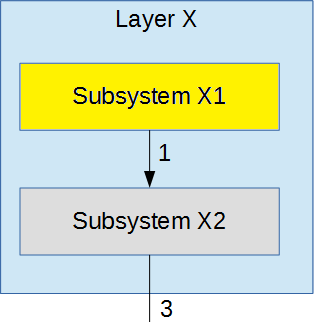
\includegraphics[width=0.60\textwidth]{images/subsystem}
 \caption{Example subsystem description diagram}
\end{figure}

\subsubsection{Subsystem Software Dependencies}
The Recipes Subsystem has no additional dependencies.

\subsubsection{Subsystem Programming Languages}
The Recipes Subsystem will be developed using, React.js, HTML, and CSS.

\subsubsection{Subsystem Data Processing}
The Recipes Subsystem will display all recipes retrieved by the Query Manager.

%------------> Meal Plan
\subsection{Meal Plan Subsystem}

\begin{figure}[h!]
	\centering
 	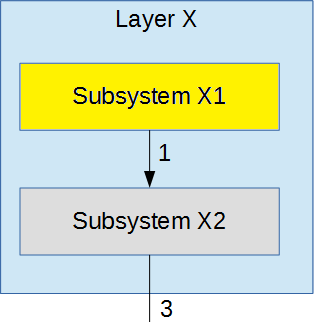
\includegraphics[width=0.60\textwidth]{images/subsystem}
 \caption{Example subsystem description diagram}
\end{figure}

\subsubsection{Subsystem Software Dependencies}
The Meal Plan Subsystem has no additional dependencies.

\subsubsection{Subsystem Programming Languages}
The Meal Plan Subsystem will be developed using, React.js, HTML, and CSS.

\subsubsection{Subsystem Data Processing}
The Meal Plan Subsystem will dislay of the current user's Meal Plans that are retrieved by the Query Manager.

%------------> Shop
\subsection{Shop Subsystem}

\begin{figure}[h!]
	\centering
 	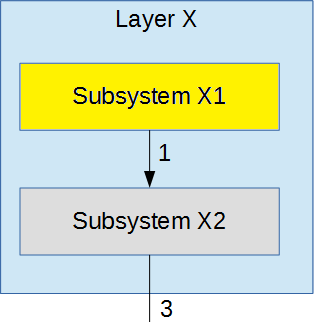
\includegraphics[width=0.60\textwidth]{images/subsystem}
 \caption{Example subsystem description diagram}
\end{figure}

\subsubsection{Subsystem Software Dependencies}
The Shop Subsystem depends on a consistent connection to the Shop Manager on the Server layer.

\subsubsection{Subsystem Programming Languages}
The Shop Subsystem will be developed using, React.js, HTML, and CSS.

\subsubsection{Subsystem Data Processing}
The Shop Subsystem will display all information that is calculated by the Shopping Manager.



\newpage
\section{Y Layer Subsystems}
In this section, the layer is described in some detail in terms of its specific subsystems. Describe each of the layers and its subsystems in a separate chapter/major subsection of this document. The content of each subsystem description should be similar. Include in this section any special considerations and/or trade-offs considered for the approach you have chosen.

\subsection{Subsystem 1}
This section should be a general description of a particular subsystem for the given layer. For most subsystems, an extract of the architectural block diagram with data flows is useful. This should consist of the subsystem being described and those subsystems with which it communicates.

\begin{figure}[h!]
	\centering
 	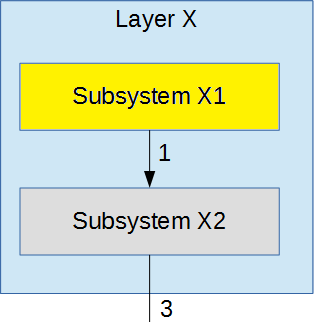
\includegraphics[width=0.60\textwidth]{images/subsystem}
 \caption{Example subsystem description diagram}
\end{figure}

\subsubsection{Assumptions}
Any assumptions made in the definition of the subsystem should be listed and described. Pay particular attention to assumptions concerning interfaces and interactions with other layers.

\subsubsection{Responsibilities}
Each of the responsibilities/features/functions/services of the subsystem as identified in the architectural summary must be expanded to more detailed responsibilities. These responsibilities form the basis for the identification of the finer-grained responsibilities of the layer's internal subsystems. Clearly describe what each subsystem does.

\subsubsection{Subsystem Interfaces}
Each of the inputs and outputs for the subsystem are defined here. Create a table with an entry for each labelled interface that connects to this subsystem. For each entry, describe any incoming and outgoing data elements will pass through this interface.

\begin {table}[H]
\caption {Subsystem interfaces} 
\begin{center}
    \begin{tabular}{ | p{1cm} | p{6cm} | p{3cm} | p{3cm} |}
    \hline
    ID & Description & Inputs & Outputs \\ \hline
    \#xx & Description of the interface/bus & \pbox{3cm}{input 1 \\ input 2} & \pbox{3cm}{output 1}  \\ \hline
    \#xx & Description of the interface/bus & \pbox{3cm}{N/A} & \pbox{3cm}{output 1}  \\ \hline
    \end{tabular}
\end{center}
\end{table}

\subsection{Subsystem 2}
Repeat for each subsystem

\subsection{Subsystem 3}
Repeat for each subsystem


\newpage
\section{Z Layer Subsystems}
Groco will  use a relational database to keep back end information uniform and well structured. There will be 5 different table subsystems. They are user table subsystem, meal plan table subsystem, brand table subsystem, ingredients table subsystem and recipe table subsystem.

\subsection{Layer Operating System}
The database layer will run on AWS. Thus, it will use whatever operating system AWS is using.

\subsection{Layer Software Dependencies}
The database layer will depend upon postgres for the creation of tables and execution of queries. Also, the database layer will depend upon Amazon Web Services(AWS) for hosting the database on the cloud. 

\begin{figure}[h!]
	\centering
 	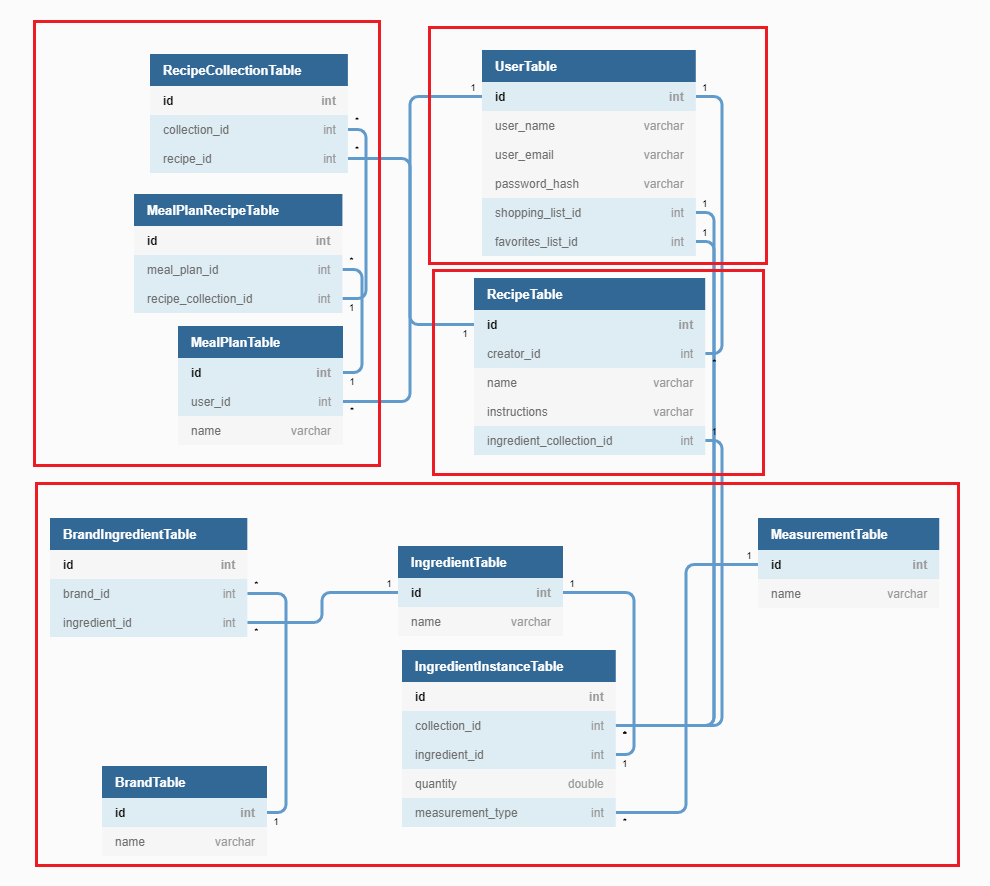
\includegraphics[width=0.60\textwidth]{images/Database.png}
 \caption{Database Diagram}
\end{figure}

\subsection{USER TABLE SUBSYSTEM }
The User table Subsystem will be used for storing identifiable information about each user and holding information to help the user. It has only one table called User table.

\begin{figure}[h!]
	\centering
 	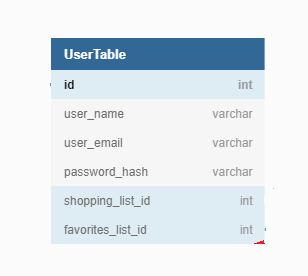
\includegraphics[width=0.60\textwidth]{images/User_Table.png}
 \caption{User Table subsystem }
\end{figure}

\subsubsection{Subsystem Software Dependencies}
User Table subsystem does not have additional dependencies.

\subsubsection{Subsystem Programming Languages}
The user table subsystem will be created using SQL and queried using SQL.

\subsubsection{Subsystem Data Processing}
Whenever a user is added to the system, their email, username, and password will be added to this table.A global ID will also be used to improve data efficiency and ensure data integrity. 

\subsection{MEAL PLAN TABLE SUBSYSTEM }
The Meal Plan Subsystem will be in charge of complying with customer requirements regarding having meal plans and related features. It has two tables called meal plan recipe table and meal plan table.

\begin{figure}[h!]
	\centering
 	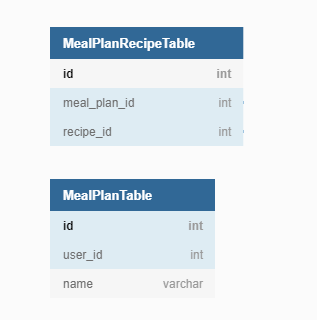
\includegraphics[width=0.60\textwidth]{images/MealPlan_SubSystem.png}
 \caption{Meal plan table subsystem diagram}
\end{figure}

\subsubsection{Subsystem Software Dependencies}
Meal plan subsystem does not have additional dependencies.

\subsubsection{Subsystem Programming Languages}
The meal plan subsystem will be created using SQL and queried using SQL.

\subsubsection{Subsystem Data Processing}
Meal plan recipe table will has mealplanid as a foreign key and it will use that foreign key when a join operation is required between meal plan recipe table and meal plan table.

\subsection{INGREDIENT TABLE SUBSYSTEM }
The Ingredients Subsystem will be used for storing ingredients required in the construction of a meal plan. This subsystem has three tables and they are called measurement table, ingredient table and ingredient instance table.

\begin{figure}[h!]
	\centering
 	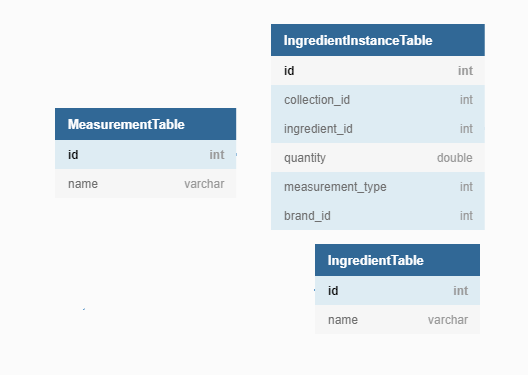
\includegraphics[width=0.60\textwidth]{images/Ingredient_SubSystempng.png}
 \caption{Ingredient Table subsystem}
\end{figure}

\subsubsection{Subsystem Software Dependencies}
Ingredient Table subsystem does not have any additional dependencies.

\subsubsection{Subsystem Programming Languages}
The user table subsystem will be created using SQL and queried using SQL.

\subsubsection{Subsystem Data Processing}
The ingredients instance table will use measurement type and ingredient id foreign keys when the join operation is required between measurement table, ingredient table and ingredient instance table.

\subsection{RECIPE TABLE SUBSYSTEM }
The Recipe Table Subsystem will responsible maintaining lists of all recipes, along with associated ingredient collection IDs. It has only one table called recipe table.

\begin{figure}[h!]
	\centering
 	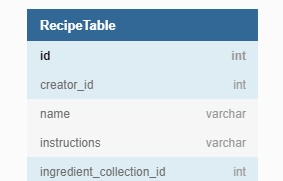
\includegraphics[width=0.60\textwidth]{images/Recepice_Subsystem.png}
 \caption{Recipe Table subsystem diagram}
\end{figure}

\subsubsection{Subsystem Software Dependencies}
Recipe Table does not have any additional dependencies.

\subsubsection{Subsystem Programming Languages}
The user table subsystem will be created using SQL and queried using SQL.


\subsection{Brand table subsystem }
The Brand Table Subsystem will responsible maintaining lists of all brands, along with associated ingredient of the brand. This subsystem has two tables: Brand Table and Brand Ingredient Table.

\begin{figure}[h!]
	\centering
 	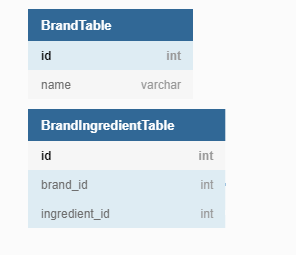
\includegraphics[width=0.60\textwidth]{images/Brand_Table.png}
 \caption{Recipe Table subsystem diagram}
\end{figure}

\subsubsection{Subsystem Software Dependencies}
Recipe Table does not have any additional dependencies.

\subsubsection{Subsystem Programming Languages}
The user table subsystem will be created using SQL and queried using SQL.

\subsubsection{Subsystem Data Processing}
Brand ingredient table has brandId as foreing key and it will be used when a join operation is required between brand table and brand ingredient table. It also has ingredient id as a foreign key which will be used when a join operation is required between brand ingredient table and ingredient table.
\newpage
\section{Data Controller Subsystems}
%In this section, the layer is described in some detail in terms of its specific subsystems. Describe each of the layers and its subsystems in a separate chapter/major subsection of this document. The content of each subsystem description should be similar. Include in this section any special considerations and/or trade-offs considered for the approach you have chosen.
The data controller layer is responsible for getting data about grocery items from different stores and transferring the data to the shopping manager subsystem which is in the Server/Back end layer. There is only one subsystem in the data controller layer, the API manager. Since many stores do not allow web scraping, the developer team decided to use APIs from stores and gather grocery data.
\subsection{API manager}
%This section should be a general description of a particular subsystem for the given layer. For most subsystems, an extract of the architectural block diagram with data flows is useful. This should consist of the subsystem being described and those subsystems with which it communicates.

\begin{figure}[h!]
	\centering
 	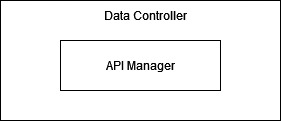
\includegraphics[width=0.60\textwidth]{images/data_controller.jpg}
 \caption{Data controller subsystem diagram}
\end{figure}

\subsubsection{Assumptions}
%Any assumptions made in the definition of the subsystem should be listed and described. Pay particular attention to assumptions concerning interfaces and interactions with other layers.
All of the stores will return grocery descriptions in JASON format. 
\subsubsection{Responsibilities}
%Each of the responsibilities/features/functions/services of the subsystem as identified in the architectural summary must be expanded to more detailed responsibilities. These responsibilities form the basis for the identification of the finer-grained responsibilities of the layer's internal subsystems. Clearly describe what each subsystem does.
The API manager will take a grocery list and give the items in the list to the stores APIs. If the store API will find the given items then it will return the description of the items else it will return an error message. After the API manager gets the data it is responsible for transferring the data to the store manager subsystem. 
\subsubsection{Subsystem Interfaces}
%Each of the inputs and outputs for the subsystem are defined here. Create a table with an entry for each labelled interface that connects to this subsystem. For each entry, describe any incoming and outgoing data elements will pass through this interface.

\begin {table}[H]
\caption {Subsystem interfaces} 
\begin{center}
    \begin{tabular}{ | p{1cm} | p{5cm} | p{3.5cm} | p{3.5cm} |}
    \hline
    ID & Description & Inputs & Outputs \\ \hline
    \#1 & The given grocery is found & \pbox{3cm}{list of grocery items} & \pbox{3cm}{grocery item descriptions}  \\ \hline
    \#2 & The given grocery is not found & \pbox{3cm}{list of grocery items} & \pbox{3cm}{not found message }  \\ \hline
    \end{tabular}
\end{center}
\end{table}

%\subsection{Subsystem 2}
%Repeat for each subsystem

%\subsection{Subsystem 3}
%Repeat for each subsystem


\newpage

%%% References
\bibliographystyle{plain}
\bibliographystyle{reference/IEEEtran_custom}
\bibliography{reference/refs}{}

\end{document}